\section{Dawn - 黎明期と達人たち}

\subsubsection*{Pocari 氏}
\noindent 全日本タイピスト連合リーダー。毎日パソコン入力コンクール技術顧問。メディアへの露出も多いタイピング界の顔。タイピングスキルは現役当時からトップレベルであり、特に和文実用入力において右に出るものはいない。
\subsubsection*{dqmaniac 氏}
\noindent 古参中の古参であり、その日記は過去のタイピング界に関する筆頭文献。分析・攻略能力が人並み外れており、文化的貢献は計り知れない。競技に対する純粋で真摯な態度も、過去から現在まで多数の競技者を刺激してやまない。
\subsubsection*{たにごん氏}
\noindent 圧倒的な実力であらゆる競技・あらゆる種目を総なめにした超実力者。あまりの人外ぶりについたあだ名が「宇宙人」。伝説が数多く残されており、現在も時折競技に参加しては衰えを知らぬ指先で桁外れの成績を残していく。
\subsubsection*{むなしい氏}
\noindent 黎明期文化の牽引者にして全日本タイピスト連合設立発起人。曰く「名前はむなしいですが本当にむなしいわけありません」。タイピング界隆盛の陰の功労者。毎パソ和文・数字六段など、文句なしの上級実力者でもある。

\question{タイピング界の礎を築いて来られた「達人」の皆さんにお目にかかれて光栄です。本日はよろしくお願いします。}

\answer{Pocari・dqmaniac・むなしい}{よろしくお願いします。}

\answer{むなしい}{「達人」と言っても、俺はたまたま時期が良かったってだけで、実力は雑魚っていう(笑)}

\question{ご謙遜を(笑)オフ会の開催など、当時の文化的な中心人物であったと伺っています。まずは、そうした競技タイピング界の黎明期、一番はじめの頃について伺おうかと思います。}

\answer{むなしい}{dq さんの時代だ。}

\answer{dqmaniac}{そもそものきっかけは 1999 年 12 月 15 日、TOD\footnote{The Typing Of the Dead}のロケテストが開始された時。その日に、多少タイピングには自信があったから、やりにいったわけだ。すると、何か知らないけど、ボッコボコにされて。 16 コイン使ってようやくクリアしたのかな。それで「やってやる!」と、火がついてしまったわけです。一方で、昔懐かしの美佳タイプ\footnote{美佳のタイプトレーナ}をたまたま検索していたら見つけたんで、TODと並行して練習し、タイピング能力を強化していこうと。}

\answer{むなしい}{その当時から美佳のランキング Typing Attack\footnote{今では消えてしまい、残っていないが、初期の文化の中心的なサイトだった。}は……。}

\answer{dqmaniac}{あった。}

\answer{むなしい}{誰が一位だったとか覚えてます?}

\answer{dqmaniac}{誰だったかな、俺の前…… CX さんかな……。}

\answer{むなしい}{すぐ自分が一位に?}

\answer{dqmaniac}{うん。}

\answer{むなしい}{じゃあもうその当時は dq さんが一位だったと。}

\question{ランキングサイト Typing Attack はそれ以前からあったというのもすごい話ですね。}

\answer{むなしい}{で、(Typing Attack のランキングは)しばらくはずっと dq さん独走の時代だよね。1999 年から始まってずっと。}

\answer{Pocari}{僕が入った頃もdq さんが一位だった。}

\answer{むなしい}{ぽかたんが入ったのはいつ?}

\answer{Pocari}{自分の日記によると……2000 年の 8 月だ。8 月 24 日、初登録。}

\answer{むなしい}{なんで始めたの、それは。}

\answer{Pocari}{それが思い出せないんだよね……元々ゲーマーだったから、タイピングはPC98時代に「クムドールの剣」というソフトで覚えて、その後も特打くらいはやっていたんだけど。なんとなく検索してた時に見つけたんじゃないかな。多分ランキングを先に見つけたんだと思う。ランキングがあるものじゃないと、やらなかっただろうから。}

\answer{むなしい}{その当時はランキングは実質的に美佳しかなかったからね。}

\answer{Pocari}{市販ゲーを除くとね。で、ランキングがあるから美佳タイプやってみようと。周囲の友達に速いねとは言われてたってのもあるかな。まぁそれは井の中の蛙的なもんだと思っていたけれど。試しに全種目一回ずつやって、登録してみたら、確か総合六位だった。でも初登録で六位ってことは、この「井」では頑張れば一位が取れるかもしれないと思い、ちょっとやり込んでみた。一位を取って「よしよしここは制したぞ」って満足しようと。ところが、ランキング上位の人の日記を見に行くと、どうもかなりやり込んでいる人(dqmaniac 氏)がいると(笑)}

\answer{一同}{(笑)}

\answer{Pocari}{そこで、これは全種目一位を目指すぞ! と気合が入った。その頃はそんなにハイレベルな場所だとは思わなくて、さくっといけるかなと思ったら、これが全然一位になれない(笑)なんだこの Yuki(dqmaniac 氏の旧ハンドル)って奴は! みたいな(笑)。特にランダム系が全然ダメで。}

\answer{むなしい}{じゃあぽかたんと dq さんが争ってた時代ってのがあったんだ。}

\answer{Pocari}{争った……っていうほど、何かがあったわけじゃないかもしれないけど、水面下で静かな戦い。当時はまだコミュニケーションもなかったしね。}

\answer{dqmaniac}{ローマ字や英単語ではあっという間に抜かれたし。}

\answer{むなしい}{俺が始めたのは 2000 年の 12 月くらいかな。元々 dq さんはドラクエやってる人でしょ。俺もそうなんだけど、ドラクエが好きで dq さんのホームページを知って、タイピングのコンテンツに影響されてタイピングを始めた人っていうのはもの凄く多い。俺以外に 100 人は軽くいると思う。美佳タイプだけど始めたころは、タッチタイピング覚えたてレベルで……けど、二ヶ月も練習すればかなりできるようになるじゃん、タイピングって。だからその頃はバンバン伸びてて、楽しいなと。}

\question{なるほど、伸びますよね。}

\answer{むなしい}{当時と今を比べるのに「これだけは言わせて」と大事な事があって。それは、当時ネット上で交流する手段が今のようにはなかったんだという事。}

\answer{Pocari}{技術的なツールという意味では、例えば自分は Mirabilis の ICQ を使ってたし、個人個人では使っていたのかもしれないけど、タイパー間をつなぐものは全くなかったね。IRC に\#TypingAttackのチャンネルができるまでは。}

\question{では当時の交流は、どのようにされていたんですか。}

\answer{dqmaniac}{Typing Attack の掲示板とかでは。}

\answer{むなしい}{も、あるんだけど、そこはあまり流行っていなくて、Ibuki さんという別な方のサイトがあって、そこの掲示板とかで。とにかく掲示板で話すしかなかったんだ。「俺今日ここまで伸びたぜー」とか。しかも当時俺らダイヤルアップ接続だったから、掲示板を一日一回確認、十秒で書き込んですぐ切る、とかそういう時代だった(笑)}

\question{時代を感じるお話ですね。}

\answer{むなしい}{そして、その頃並行して、dq さんが日記で TOD のことをバンバン書いていた。}

\question{TOD はロケテスト後にすぐ正式稼働したんでしたっけ。}

\answer{dqmaniac}{正式稼働が 2000 年 1 月。この時は旧 ROM と呼ばれている、難しいやつで。4 月になってようやく、新 ROM(今出回っている難易度が落ちたバージョン)になった。その辺りからワンコインクリアできる人達が増えてきて、メジャーになっていった。}

\answer{むなしい}{なので 2001 年に入る頃にはもうその掲示板では「美佳タイプ今日はこれくらい伸びた」とか「TOD を 3 コインでクリアできるようになった」という話で盛り上がってた。そして「オフ会しませんか」という話が掲示板で出て、その Ibuki さんのサイトにいた人達で 3 月 10 日に集まった。(それ以前にも数名規模のごく小規模なオフはあったが)これが初めての大規模なオフ。}

\question{「秋葉原パセラオフ」と呼ばれている有名なオフですね。}

\answer{むなしい}{今まで速い人とか実際に見たことがなかったから、見るだけでもすごく新鮮だったし。あとは TOD の対戦だ。対戦の良さを言葉で説明するのはすごく難しいんだけど……これをきっかけに TOD オフが一気に大ブームになった。}

\answer{dqmaniac}{この頃は「オフ会」というとほぼすべて TOD で対戦ということを意味していた。}

\answer{むなしい}{ゲーセンで集まって、TOD は 2 台くらいしかないから対戦者以外は後ろで観戦しているっていう。5 時間くらいぶっ通しで十数人が立ちっぱなしで台を囲んでいる、今振り返ると異様な光景だったと思う(笑)}

\answer{dqmaniac}{メシを食いに行ったら、そこでまた 3 時間くらいぶっ通しでタイピングトークをしているわけだ。}

\answer{むなしい}{タイプウェルの話とか美佳タイプの話をね。}

\question{それがきっかけになってオフ会文化というのが広がっていったんですね。}

\answer{むなしい}{この後は定期的に、月に一回とかそれくらいやってた。俺がいつも自分のホームページ上でアナウンスして、幹事をやって。}

\question{むなしいさんが大活躍されるんですね。}

\answer{Pocari}{超大活躍してたよ。当時オフの主催はほとんどむなしいだったんじゃないかな。}

\answer{むなしい}{東京だけじゃ物足りないから、東京の人を連れて、みんなで関西へ行ったり。そういう企画もしたよ。当時関西の人は(オフが東京で開催されるので)ショボーンだったからね。……というのが最初の1年かな。}

\question{短期間にそこまで行われていたんですね。}

\answer{むなしい}{やっぱ最初は新鮮で楽しかったから。で、一気に燃え尽きちゃうんだけど、結局は(笑)}

\answer{Pocari}{当時はまだみんな学生で、時間もあったしね。}

\answer{dqmaniac}{あとは、ゲーセンやネットカフェ、店とかでタイピングゲームの大会があるとなると、誘い合わせて行ってみたりもしたね。}

\answer{むなしい}{この頃は大会がたくさんあったよね。新宿ソフマップで TOD の大会があったりとか。あとは、タイピングサミット。}

\answer{dqmaniac}{当時小学生のあきうめ君も(秋葉原パセラ)オフに参加していて、小さい手でようやくローマ字を覚えたばかりだというのに、何なんだこの速さ! っていう。でも準決勝でKeNoに完敗して、それで本人とお父さん(父・信仁さん)に火がついてしまって(笑)}

\answer{むなしい}{当時からすごく速かった。それで信仁さんの家でオフ会をやるよということになったのが、タイピングサミットと呼ばれるオフ会(2001 年 11 月)。}

\question{今現役の人にも馴染みが深いと思うので、当時のタイプウェルのお話を少し伺いたいですね。}

\answer{dqmaniac}{タイプウェルは初期は「のみ」と「混在」しかなくて。たけひささんという当時圧倒的に強い人がいた。その後は2000年7月に英単語がリリース。11月に国語Rで、国語Kは2001年3月かな。今の形のオリジナルも2001年1月。}

\answer{むなしい}{当時はみんな美佳命って感じだったけど、だんだんタイプウェルにシフトしていったよね。ソフトの出来が当時からすごい良かったから。}

\answer{Pocari}{不正にすごく厳しいっていうのも大きな理由だった。}

\answer{むなしい}{美佳タイプ(のランキング Typing Attack)は自分で数字を入力して登録するからね(笑)}

\answer{Pocari}{なんとでも不正できちゃう仕組みだったよね(笑)その点、タイプウェルは素晴らしかった。仮に不正ができても、厳格に対処していく GANGAS さんの運営の姿勢がすごく良かった。}

\question{今の人も共感するところかと思います。}

\answer{むなしい}{この頃のコミュニケーションツールはどうだったっけ。メッセ\footnote{MSN Messenger}はかなり近いけどまだ浸透していなかったんだよ。それに、この頃はまだ常時接続じゃなかったし。}

\answer{Pocari}{コミュニケーションツール(の移り変わり)は ADSL の普及時期と連動してると思う。常時接続が普及してから、メッセでやり取りするようになっていったんじゃないかな。}

\answer{むなしい}{俺は 2001 年の 12 月に家の回線が常時接続になって、タイピングやめたんだもん。「俺はもうメッセで女を釣る方に入る」って言って(笑)}

\answer{Pocari}{ここ試験に出るんで、ちゃんと載せないとね(笑)}

\question{時系列的にはこの頃(2002 年 1-2 月)第1回毎パソもあります。}

\answer{むなしい}{当時としては「特打大会」とかと同じような感覚だったよね。出ても話題にすらならなかった。出て優勝してもそれは当たり前じゃねーかと。}

\answer{Pocari}{そうそう、タイピングゲームの大会と同じ感覚だった。あんまり盛り上がってなかったよね。}

\question{毎パソと全タ連に関しては後で詳しく伺おうと思います。その他というと……。}

\answer{むなしい}{2002 年にウェザタイ\footnote{Weather Typing}ができた。できたっていうか、元々あったんだけど、新機能としてロビー\footnote{チャット機能と対戦機能を兼ね備えたコミュニケーションツール。}ができた。それで一気にコミュニケーションが取りやすくなったよね。ウェザタイで対戦したり、ウェザタイ関係のオフもやったり。}

\answer{Pocari}{ウェザタイオフは chuuichi さん主催で、三回くらいやってたかな。ホームページを作って公に告知していたから、結構知らない人も集まっていたね。タイピングサミットを除けば、大規模なオフは当時ウェザタイオフくらいだったこともあって、盛り上がったね。}

\answer{むなしい}{ウェザタイオフは誰でも参加できたしね。サミットは元々信仁さんと関わりのある方を呼ぶという形だったから。}

\answer{Pocari}{あとオフ会的なことというと、ルパン\footnote{ルパン三世 THE TYPING}が出た時(2002年4月)は、池袋 GIGO に行けば誰かいるみたいな状況だった。}

\answer{むなしい}{しかしルパンは、対戦システムが微妙で盛り上がらなくて……。 TOD の後釜で出たゲームだったから期待していた分、ショックが大きかった。}

\answer{dqmaniac}{ルパンオフと言いつつ結局 TOD 対戦やってたよね。}

\answer{Pocari・むなしい}{そうそうそうそう(笑)}

\answer{Pocari}{TOD と言えば、この頃に SEGA の話が。}

\question{公式に「達人(エキスパート)」としてプロジェクトに参加されたときですね。}

\answer{Pocari}{まずメールが dq さんと僕に来たんです。SEGA の小堤さんというプロデューサーの方から。}

\answer{dqmaniac}{2002 年の8 月。「TOD2003 というゲームを企画しています。是非とも協力して下さい」と。ぽかたんと俺、2 名しかアクティブなタイパーを知らないので、他にアクティブでやり込んでいる方がいたら紹介してください、とも。}

\answer{Pocari}{これは拡散しないと、って思っていたところに dq さんからメールが来たから、お任せして、僕は単に参加表明をしたんです。dq さんがあと他に 6 人くらいに声をかけて。}

\answer{dqmaniac}{基準は「TOD 対戦で俺をボコったことがある人」(声をかけて集まったのは、あきうめ・MADRIGAL・かり~・Jin・KeNo・むなしい の各氏)。}

\answer{一同}{(笑)}

\answer{dqmaniac}{それで、オフ会と称して関東圏で会える人だけ会おうという話になって。}

\answer{Pocari}{むなの日記にも書いてあるよね、「達人オフ」とかって面白おかしく。}

\answer{dqmaniac}{10月にはあきうめ君も京都から関東に来て、SEGA 本社で色々とやったわけです。}

\answer{Pocari}{当時は発売まで伏せていたからね。多分 dq さんの日記も伏せて書いてあると思う。そのころの日記で、あきうめ君が来ているオフがあれば、間違いなくそれです。}

\question{具体的にどのように関わられたんでしょう。}

\answer{むなしい}{自分らで数字(各種パラメータ)を弄って調整したんだよね。}

\answer{Pocari}{ini ファイル\footnote{パラメータの設定ファイル。}が直接編集できる形になっていて。ゲームの中の自分と闘いながら、実際の自分とほぼ同じ能力になるように「後半加速」とか「クイズ正解率」とかをアジャストしていって。あんまりデフォルメみたいなこともしなかった気がする。}

\answer{むなしい}{と、これをやっているとほぼ同時期に、テレビ出演があったんだよね。タイミングよく時期がかぶっていて。}

\question{「タモリのグッジョブ!」ですね。}

\answer{dqmaniac}{テレビの話はいつ来たんだっけ。}

\answer{Pocari}{グッジョブの初回放送は 2002 年 10 月 21 日、だからそのちょっと前かな。}

\answer{dqmaniac}{毎パソ経由でぽかたんに話が行ったとか。}

\answer{Pocari}{そう、「日本一の人を紹介して」という話がまず毎パソに来て、それが僕の所に来た。当初は出るかどうか結構悩んだんです。グッジョブより前にいくつか番組の出演はあったんだけど、それは朝のニュースとかで、時間も短かったし、いいかなぁって感じだった。対して、グッジョブは夜で、バラエティでしょ。でも、撮影も休みに合わせてくれるというし、タイピングを広めるチャンスでもあるし、ここは思い切って出てみるか、と思って。}

\answer{むなしい}{一番最初は、ぽかたんがたった一人で闘打をやったやつだよね。ジョーの。}

\answer{Pocari}{そう、「あしたのジョー闘打」ってやつを一人で。それが第1回だね。……で、そしたら視聴率が思いの外、良かった。タイピングのシーンが瞬間最高視聴率で、奇跡の 10\% 超え! みたいな。嬉々として電話がテレビ局からかかってきて、「すばらしいですねタイピング! 最高ですねタイピング! 僕も始めます!」と(笑)}

\answer{一同}{(笑)}

\answer{Pocari}{当然、なんとか続投したいという話になった。当時僕は忙しくて、他の方に回したかったんですけど、あちらは「対戦」という形で盛り上げたいということで……「じゃあ対戦できるゲーム(TOD)があるので」と僕から申し上げて。SEGA ともちょうど TOD2003 エキスパートの件でつながりがあったので、相談すればなんとかなるかなと。}

\answer{むなしい}{本当にタイミング良くかぶっていて(笑)}

\answer{Pocari}{相手はウェザタイのロビーで探せばいいやと思ったんですけど、当時僕と実力が拮抗してた MADRIGAL に断られてしまったり、撮影が一週間後とかに迫っていたりで、困った。困っていたところ、そういえば、すぐに来てくれそうな奴が一人いるな、と思って(笑)}

\answer{むなしい}{俺(笑)}

\question{なるほど(笑)}

\answer{Pocari}{それからSEGAにも連絡して、TOD利用の許可を取った。}

\answer{むなしい}{SEGA としてはもの凄くおいしい話だよね。すごいコマーシャルになるので。}

\answer{Pocari}{うん。むしろ「ソフトウェアの改修とか必要だったらやりますよ!」とかそういう状態で(笑)}

\answer{むなしい}{で、もう、すぐ次の日とかにうちにテレビ局が来て。当時のテレビを見てもらえばわかるけど、挑戦状とか書くんだよ。}

\answer{Pocari}{書いてないでしょ(笑)}

\answer{むなしい}{挑戦状は俺がタイピングやってる隣で AD が書いて(笑)ぽかたんが「受けて立ちますよ!」とか言ってるんですけど、あれも俺、後ろで見てたし。}

\answer{一同}{(笑)}

\question{テレビってそんなものですよね(笑)}

\answer{むなしい}{もっと言えば、dq さんが出たときに「私はこんな職場で働いています」って紹介があるんですけど。}

\answer{dqmaniac}{あのオフィスは SEGA で、ADが上司役をやってました。}

\answer{一同}{(笑)}

\answer{Pocari}{第2回の時にはまだ第3回・第4回という話は出ていなくて。第2回を撮って、放送してみたら……これまた最高視聴率。それも、その番組の中でじゃなくて、その帯の中での最高視聴率だった。}

\answer{むなしい}{最高視聴率 17.7\%! 今なら、CM出演が来るレベル(笑)}

\answer{Pocari}{あれは……番組が野球中継で 35 分くらい遅れていて、ちょうどタイピングのシーンが 23 時過ぎになった。そこで、多分 23 時のニュース番組を見ようと思ってテレビをつけた人が見たんだと思う(笑)あの時間帯の枠ではありえない視聴率が出て、それはもう持ち上げられまくって。次やりましょう、次やりましょうと(笑)}

\answer{むなしい}{やべっちの発言だったかで「これどんどん対戦したら面白いんちゃう?」「次行けるでしょう」とかもあったし。}

\answer{Pocari}{すぐにまた電話がかかってきて、「次対戦できる人いませんかね!?」と。}

\answer{むなしい}{そういう話題もスタッフと既にしてたんだよね。あきうめ君がすごくいいですよ、と俺らが推したり。}

\answer{Pocari}{あきうめ君を推したのはこっちだったね。あちらは「女性がいい」と。あと僕はずっとたにごんを呼びたかったんだけど、連絡がつかなかった。で、僕らの中で女性といえば YAME さんだということで声をかけて。けっこう電話口で悩まれた気がするんですが、(夫である)Jin さんが「出ろ」と言って出てくれることになり(笑)次の回であきうめ君も出ることができて。第3回・第4回もやはり視聴率は番組内トップだったと思う。}

\question{すごいですね。}

\answer{Pocari}{当然コーナーは続投。ところが、ここで個人的に問題発生。グッジョブは撮影が土日だったんだけど、当時僕が働いていた実家の和菓子屋は、土日が超忙しかった。だから結構揉めちゃって……「これはタイピングを広める、そして自分より速いタイパーを発掘できる絶好のチャンスなんだ!」と粘ってみた。けれど、第4回でとうとうダメになってしまって、「お仕事の都合」ということで引退しました。引退するからには、それなりの人に引き継がなきゃいけない、それなら dq さんしかいない。そういうわけでコンタクトを取って、dq さんから快諾を頂きました。dq さん、その頃の心境というのは。}

\answer{dqmaniac}{色んな知り合いがテレビに出てるから、俺も出てみてーなとは思っていて。挑戦者募集もやってたから、応募しようかとも考えて……そんな瞬間にぽかたんから連絡が来た。}

\answer{Pocari}{dq さんからガチで応募が来てたらびっくりするな、挑戦者・中山さん(dqmaniac 氏)です、って(笑)}

\answer{むなしい}{でも結局その後は、あまり続かなくて終わっちゃったんだっけ。}

\answer{Pocari}{そう。僕はその後はあんまりウォッチしてなかったんだけど…… dq さんは、たしか女性と対戦してたよね。}

\answer{dqmaniac}{まず一般で応募してきた、ごく一般的にちょっとタイピングが速い主婦の方と対戦したんです。}

\answer{むなしい}{フルボッコに(笑)}

\answer{dqmaniac}{その方が唯一、一般からちゃんと応募してきた人だったんだけど、結果はフルボッコになってしまったと。次は速い人誰かいないかという話になって、KeNo が(また Pocari 氏の紹介で)出てきた。そのガチバトルが放映されたのが 2003 年の 1 月かな。良い勝負になったけど、俺は負けてしまって、そこからはKeNoが引き継いだ。}

\answer{Pocari}{あとは chuuichi さんが、彼は確か一般から応募して通って、出たんですけど……その後くらいからタイピングから電卓になっちゃったんだよね。}

\answer{むなしい}{企画が迷走しだしてて(笑)}

\answer{Pocari}{最後は2003年3月に番組自体が終了になってしまった。}

\question{ありがとうございました。これでお話が 2003 年まで進みました。そしてこの年の毎パソ(第3回)からは全タ連として団体参加されることになりますね。全タ連(全日本タイピスト連合)設立の動機・経緯について伺いたいです。}

\answer{Pocari}{毎パソは、僕とdqさんが第1回から参加してたんですけど、ネットランキングの上位にいるようなタイパーは全然参加していなくて、ちょっとレベルが低すぎた。って言っても、当時の僕らには毎パソは事前に練習していくものという意識がなくて、初見でチャレンジしたら、和文で一般人に負けちゃったんですけど(笑)でもまあ、英文は一位二位と三位以降のスコア差がすごく開いてた。全国規模の大会なんてなかなか無いから、せっかくならレベルを高くしたいなと思って、他の人にも参加して欲しいよねって話を、むなとしてたんです。そこで「団体参加すればいいじゃん」という案が出た。その頃は定期的にタイパーのオフがあったので、その場で「団体で出ようと思ってるんだけど」とみんなに声をかけてみたのが始まり。}

\answer{むなしい}{最初はそれこそ、もう三人で団体にしようかと思ってたんだ。(参加が三人以上かつ、七部門以上が必要といった条件があったので)ぽかたんと俺で、五種目くらいずつ出て(笑)}

\answer{Pocari}{あったあった、ホームポジション部門から数字部門まで、一人で五種目行くわ、みたいな(笑)}

\answer{むなしい}{三人目は架空の名前で申し込もうぜとか(笑)最初は本当にそこからスタートだった。そもそも第1回と第2回は、(タイパーからは)ぽかたんと、dq さんと、KeNo しか出てなかったし。個人参加だと参加費も結構高くて(1部門2000円)、めんどくさいんだよね。}

\answer{Pocari}{そう、学生の方だと、送金手段がわからないとかもあって。手続きが煩雑。}

\answer{dqmaniac}{本名に加えて学校名も出ちゃうから、普段ハンドルネームで交流している人にとっては抵抗もあったしね。}

\answer{Pocari}{お金がないから参加しませんという人も多かった(笑)団体で出ると一人 700 円なので、かなり安くなる。}

\answer{むなしい}{なので(自分たち二名と架空の一名で作っちゃおうかな、なんていう)下らない話をしながら、オフで声をかけてみたら、意外と俺もやるよ俺もやるよって人がいて。その場でもういきなり十何人かゲット。}

\answer{Pocari}{で、その場で団体の名前を決めようって流れになった。ぱっと考えるの難しいから……ウェザタイってワードが前半と後半で分かれていて、ランダムでくっついて出題されるじゃないですか。あれの真似をして、前半と後半に分けて考えようとした。形容詞と名詞、みたいな感じに。色々出たよね。「全日本」も当然入っていたし「炎の」とか「一にも二にも」とか(笑)後半部分ももちろん色々候補があって、「タイピング」「タイパー」「タイピスト」「打鍵者」、「Kiss」もあった(笑)「一にも二にもKiss」(笑)}

\answer{一同}{(笑)}

\answer{Pocari}{本当にそれになりかねたからね、危うく(笑)ほぼ全員賛成状態だったんだけど、間一髪「いやちょっとこれ、運営側に止められるかもしれない」という意見が出て、無難どころで「全日本タイピスト連合」っていう名前になりました。}

\question{最終的に立派な名前なので、そんな面白おかしい経緯があるとは存じませんでした(笑)「タイパー」でなく「タイピスト」である理由というのはあるんでしょうか。}

\answer{Pocari}{前半・後半の組み合わせで語呂が良さそうなものに決めただけなんだけど、(毎パソは)変換を伴うので単あるゲームじゃないってイメージがあって、正確性もすごく重要なので、実用っぽい言葉の「タイピスト」の方が合うんじゃって感じで。なんとなく、カッコイイっていう僕の中でのイメージもあったんですけど。}

\answer{むなしい}{「タイパー」と「タイピスト」の違いはなんぞや、とかいう話を当時色々していた記憶があるね。「タイパー」はゲームっぽい、とかいう話があったね。「タイピスト」は実用っぽい、みたいな。}

\question{当時からこの話題っていうのはあったんですね。}

\answer{むなしい}{うん。でも、名前とかが決まっても、当時基本的には俺と dq さんとぽかたんが中核となってやってたんだ。最初は(全タ連の)ページも俺のウェブスペース上にふざけたのがあっただけだったし。他の人は名前だけ貸すみたいな感じで。そんなに練習もしないで本番だけ出ますよーとか、そういう人も多かった。}

\answer{Pocari}{団体で出るメリットって何だろうと考えて、コンセプトは早い段階で決めました。「目立つ」「安くなる」「団結心」「思い出」。学生が多かったから「高校生以下は無料」っていう独自制度も作ったり。}

\answer{むなしい}{でも当時は毎パソなんて……しょっぱい大会というか、みんなタイプウェル命だったので。ウェザタイも盛んに……盛んにチャットをしてた(笑)そんな感じで、毎パソも団体で参加してみたはいいものの、ほとんどの人はやる気ない状態だった。}

\answer{Pocari}{やる気ない人が多かった理由のひとつが「各予選の上位 50 位まで決勝に参加できる」ってルールだったと思う\footnote{今は上位5位まで。}。ほとんどのタイパーは参加すれば予選通過は楽勝だったので、練習しようという気が起きなかったんじゃないかな。僕も第1回・第2回は練習をしようなんて発想もなかった。例えていうなら、「明日『宇宙戦艦ヤマトタイピング』の大会があります」と聞いたって、買って練習まではしませんよね(笑)そんな感じだった。}

\answer{むなしい}{でも第3回からは結構練習したんだよね。ぽかたん家に泊まって練習したり(笑)なんで練習に火がついたのかは、よく覚えてないんだけど。}

\answer{Pocari}{一人一人理由は違うとは思うんだけど、僕は団体参加による「団結心」が大きかった。個人的に、和文で(非タイパーに)負けていたこともあって、これはちょっとまずいぞと思った。連合で出るからには一位に連合の名前を連ねたい、っていう想いが急に出てきたね。}

\question{その頃から課題文暗記などの攻略が始まったのですか。}

\answer{Pocari}{第3回に暗記をしたのは YAME さんだけじゃなかったかな……。}

\answer{dqmaniac}{いや、俺も暗記した。第3回の英文からやった。}

\answer{Pocari}{そっか。じゃあ僕は第4回からかな。はじめは暗記なんてあり得ない! って思ったけど、やってみたら意外とそこまで難しくはなかった。}

\answer{むなしい}{おかげで第3回が盛り上がって、それからは、格調高い……じゃないけど、タイパーの中で認められる大会にはなっていったよね。}

\begin{figure*}
 \begin{center}
   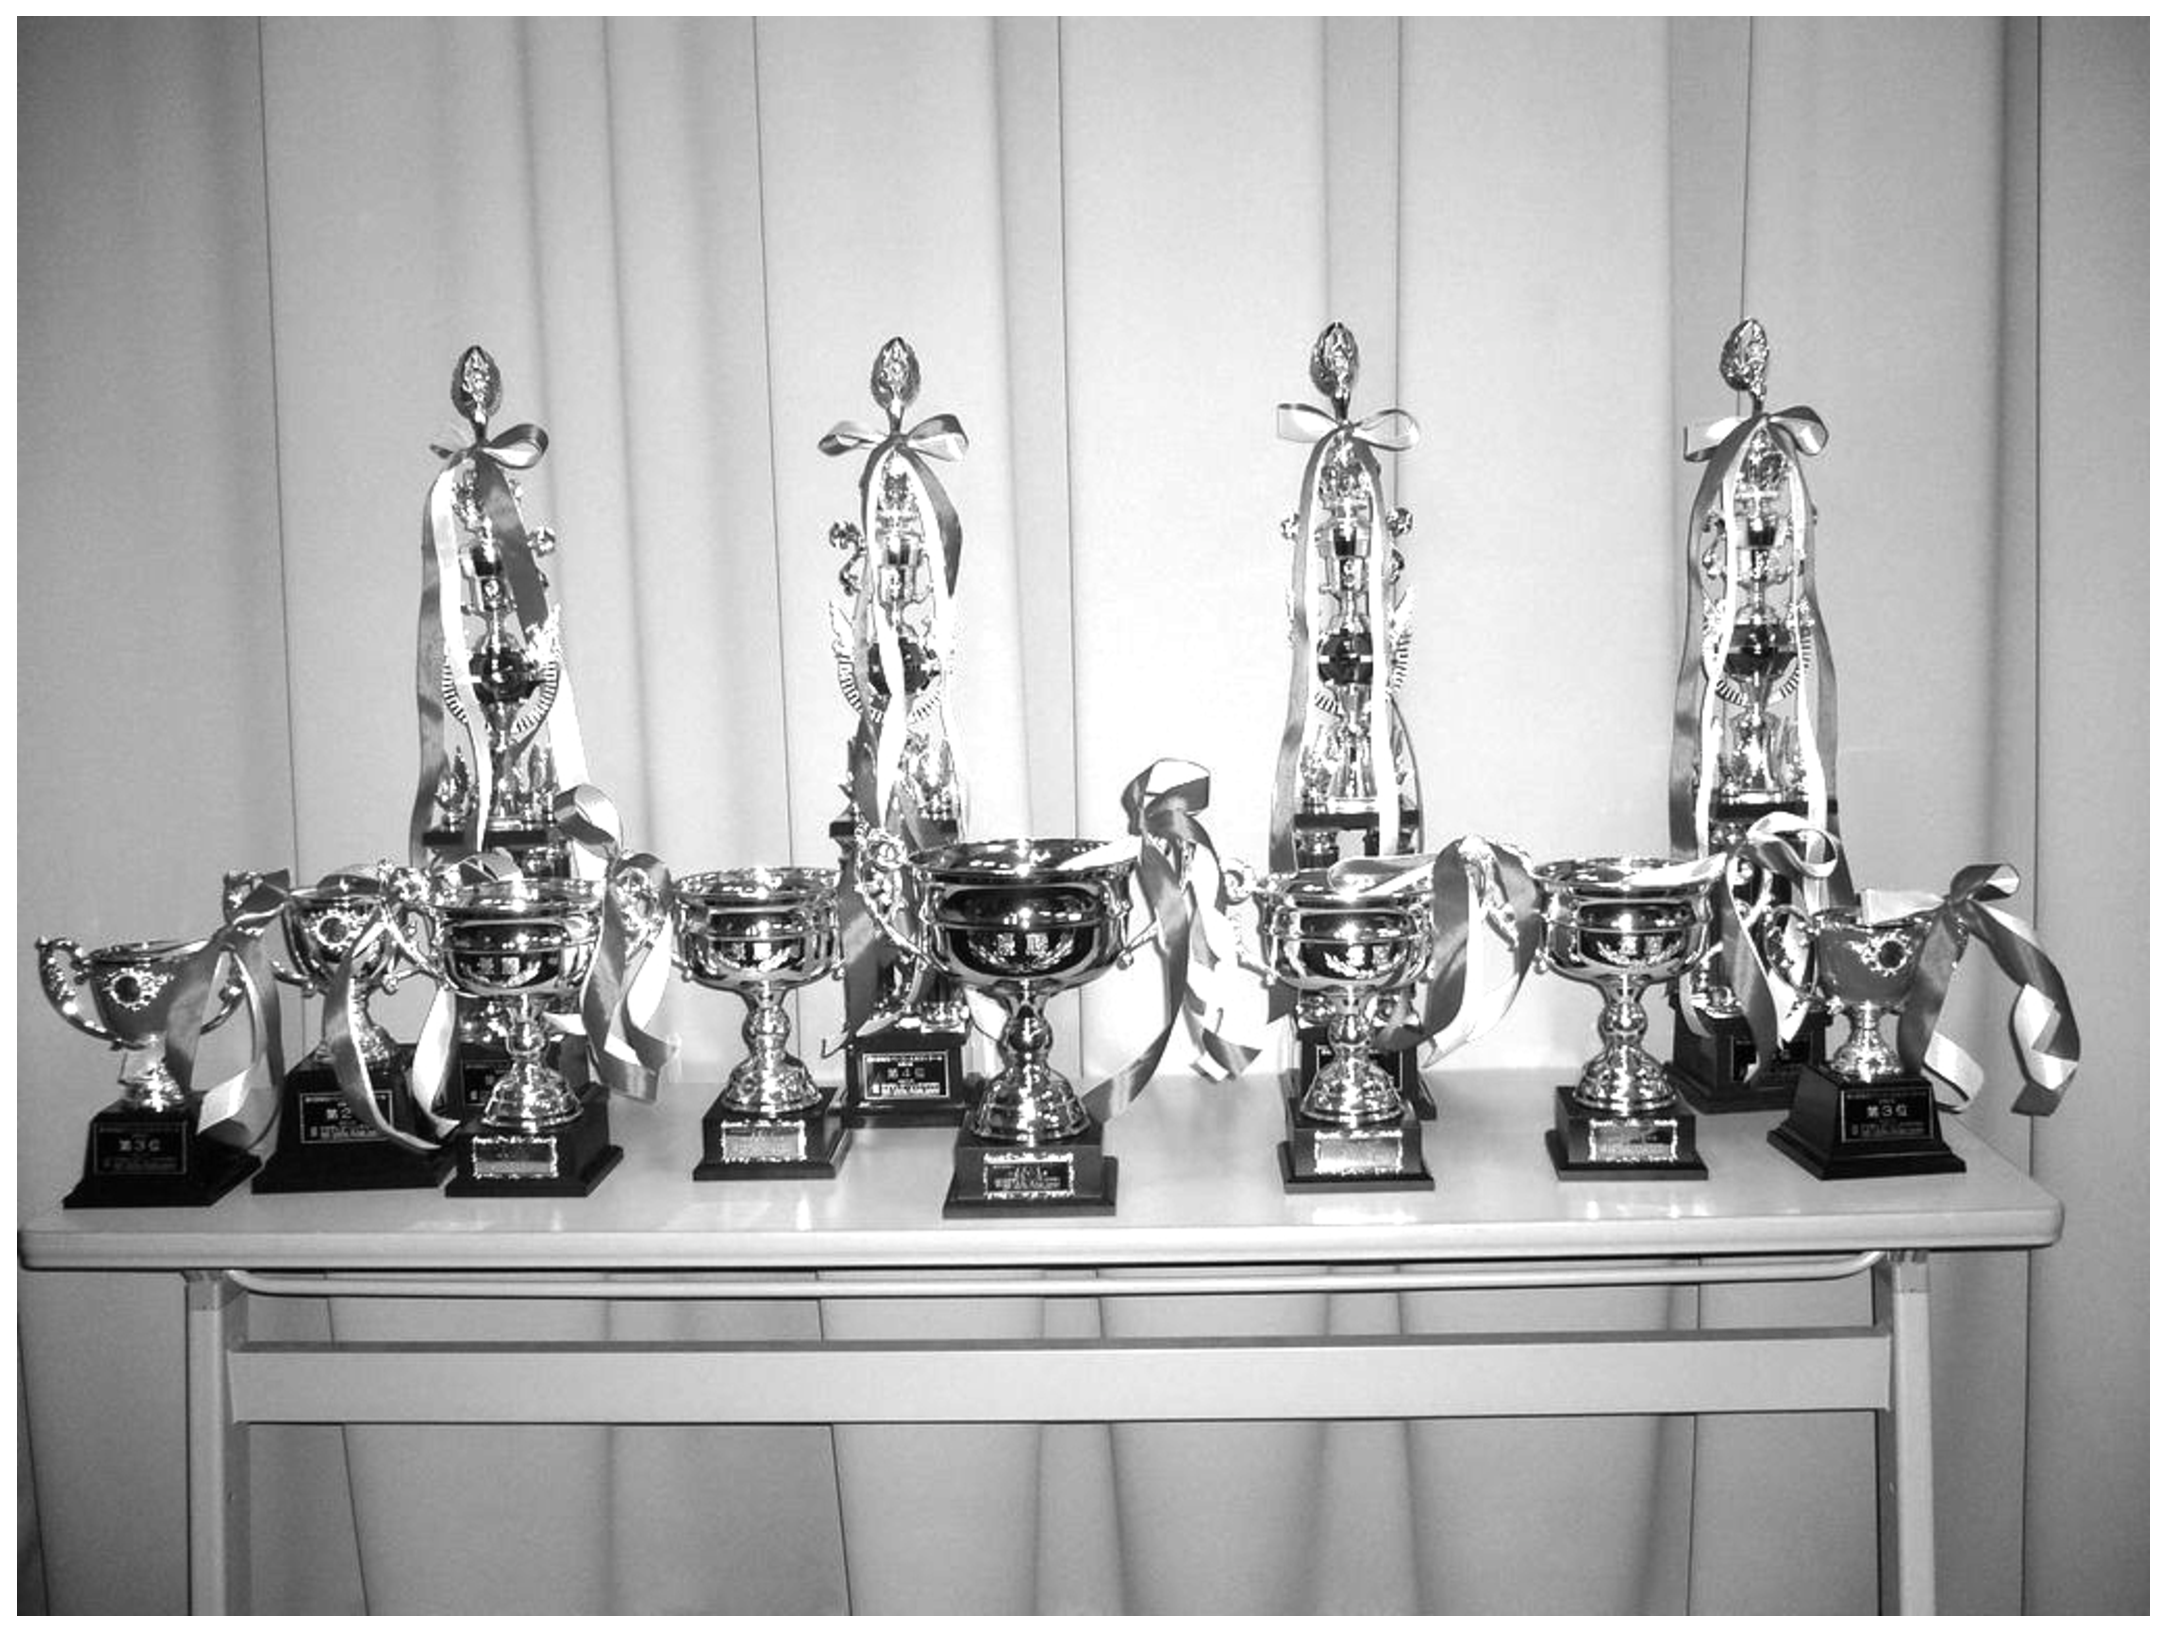
\includegraphics[width=14cm,clip]{res_x_i/typist1.eps}
 \end{center}
 \caption{第6回毎パソにて、全タ連の獲得トロフィー大集合}
 \label{trophy}
\end{figure*}

\answer{Pocari}{第3回には連合から 30 名弱参加したのかな。第4回もブームが続いて50名近くが連合から参加。全部で七部門くらいある中で、五部門くらいは連合が上位を独占してた。連合の名前が並んでいて、団体参加いいねー! って感じた。}

\answer{dqmaniac}{表彰式でみんながトロフィーをもらって、それを集めるとすごい数だった(笑)}

\answer{Pocari}{とても良い時代だったんだけれど、残念ながら第8回(2008年)から一般(大学生以上)が全国大会に参加できなくなってしまい、それからは一気に下火になっていった。}

\answer{むなしい}{大分話したけど、ここまでくらいが「黎明期」と言える時期じゃないかな。連合ができるくらいまでが。}

\answer{Pocari}{そうだね。連合を作った時の僕の日記を読み返すと「タイピング界の裾野を広げたい」みたいな言葉が出てるから、この頃からコミュニティがちゃんとできてきて、それを広めようということに意識が行ったんだと思う。}

\question{「連合ができる」という明確な区切りまでを「黎明期」とするのは良いかもしれませんね。あと、これは余談になるかもしれないんですが、これ以後、全タ連に「登山部」なるものが出来て、そちらが盛り上がっていると伺っています。}

\answer{Pocari}{むしろ僕らはもう登山部としてしか活動していないかも……(笑)登山部の活動は、2006年7月に行った名古屋の「マウンテン」にたち返ります。}

\answer{dqmaniac}{甘口抹茶小倉スパとか、メロンスパとか、要はスパゲッティが出てくる店なんだけども、その量・味がハンパじゃない。}

\question{本当にそういう味なんですか。}

\answer{Pocari}{そう、本当にメロンの味。それが食べたくて人が集まるっていう、ちょっと物珍しい店。そこにタイパーで行ったことがあって……店の名前が「マウンテン」だったので、本当の山も登りたいねなんて話をしてたんです。でも当時の僕らは皆インドア派、夢物語でした。その後、僕と友達と dq さんとで食事をしていた時に、一人登山経験者がいて、僕と dq さんがなぜか「登山いいっすね!」となった(笑)時期も良かったので、あっさり高尾山行きが決まりました。}

\answer{dqmaniac}{高尾山というと本格的な装備も不要で、ハイキング感覚で気軽に行けると教えてもらった。実際に登ってみるとその通りであり、爽快感があった。}

\answer{Pocari}{そこからは順調で、高尾山に行った時に「次は富士山だ」と目標が決まった。以後 dq さんと会う度に山の話をするようになり、むなが実は登山経験者、なんてことわかり。練習で丹沢に行き、男体山に行き、富士山です。その過程で他の方にも声をかけました。}

\begin{figure*}
 \begin{center}
   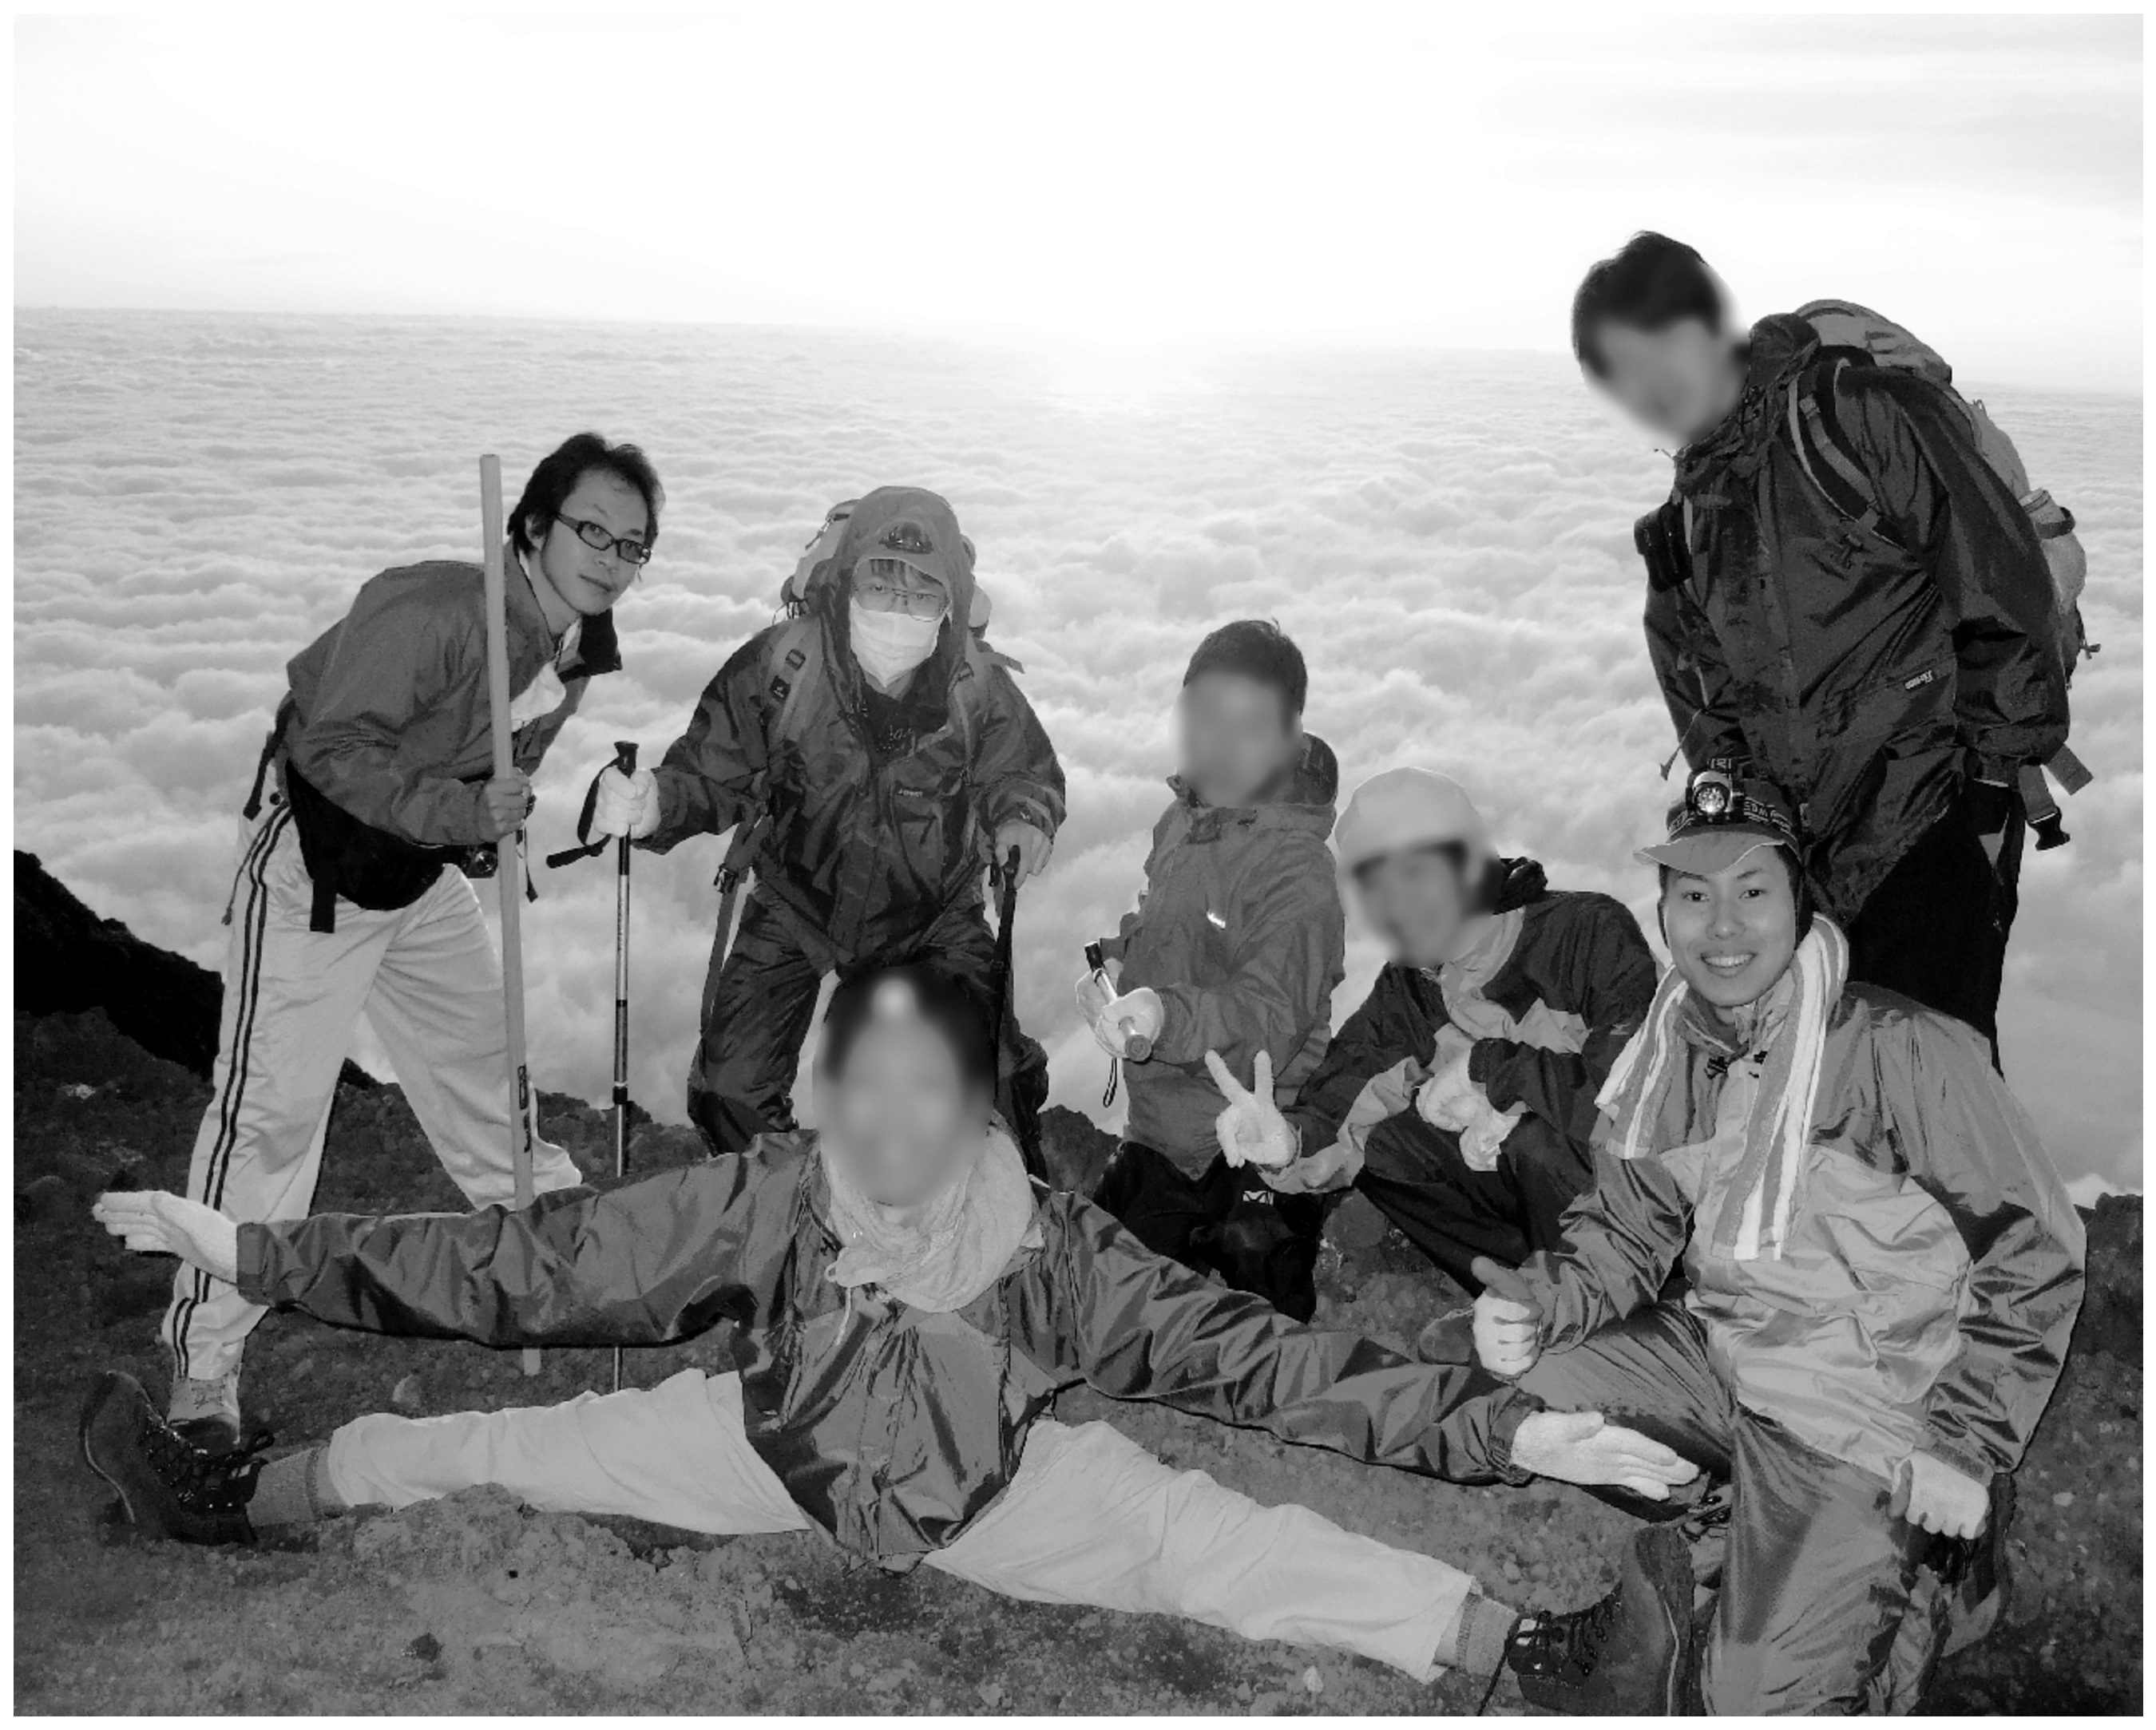
\includegraphics[width=14cm,clip]{res_x_i/typist2.eps}
 \end{center}
 \caption{富士山・山頂付近にて。左からむなしい、dqmaniac、Pocari 各氏。}
 \label{fuji}
\end{figure*}

\answer{dqmaniac}{何しろ富士山を登るにしても初心者の集まりだから、何もわかんないわけ。これはヤバいと思って、色々調べて、丹沢とか男体山とかで練習をしようと。丹沢に登る前に道具を買い、準備をしました。}

\answer{むなしい}{富士山に行ってからは、定期的に毎年一山、みたいな感じで。}

\answer{Pocari}{翌年(2009年8月)は槍ヶ岳に登ったよね。その帰り道に「いつかはキリマンジャロくらいじゃないですかね!」みたいな話をして、その年の 12 月に、これは個人的にですけど、僕はいきなりキリマンジャロに行くことに決め、行ってきました。}

\answer{dqmaniac}{ぽかたんが(キリマンジャロに)登ったっていうのに非常に刺激を受けまして、俺も翌年のゴールデンウィークに行きました。}

\answer{むなしい}{基本的にこの活動って、来る者拒まずなんだけど……富士山以来一人も増えてないんだよね。}

\answer{Pocari}{行く山が名前だけ聞くとだんだん難易度の高い山になっていってるから、入りづらいっていうのはあると思う(笑)あと僕らが積極的には勧誘をしてないってのもあるかな。}

\answer{むなしい}{もっと簡単な山に一緒に行きたい人~ってやれば、出てくるのかもしれない。}

\answer{Pocari}{この本に望みをかけてます(笑)往路でも復路でも宿でも、タイピングの昔話を楽しんだりしています。登っている間も最適化の話で盛り上がったりとか。タイパーの皆さん、ぜひ一緒に登りましょう!}

\answer{dqmaniac}{帰り道についでに TOD 対戦やったこともあったよね。タイピングと登山は、どちらも頑張って努力してやっていればだんだん強くなっていって、どんどん高い山に登れるようになる。そういう面が似てるんだろうなと。}

\answer{むなしい}{タイパーは基本的にマゾが多いから、向いてると思うよ登山(笑)}

\question{複数の趣味を共有できる仲間って楽しいだろうと思いますね。勧誘の成功を祈ります(笑)}

\answer{たにごん}{こんばんはー。}

\answer{Pocari}{お、お疲れさま!}

\question{ちょうど良いところに! タイトなスケジュールの中お時間を頂き恐縮です。よろしくお願いします。}

\answer{たにごん}{よろしくっす。}

\question{たにごんさんが合流された所で、黎明期のお話と時系列的にはややかぶりますが、2002 年から 2003 年頃の、Pocari さんとたにごんさんのタイプウェル国語 R デッドヒート時代のお話など伺えたらと思います。}

\answer{Pocari}{僕の最終更新が 2003 年 9 月だったかな。}

\answer{たにごん}{俺もそれくらいでフェードアウトした(笑)}

\answer{Pocari}{ほぼ同時期なんだよね。}

\question{お互いにそれぞれ事情があってということだったのですか。}

\answer{たにごん}{俺はプライベートの都合で全然家でタイピングできないんでフェードアウトして。}

\answer{Pocari}{僕も職が変わった頃で、忙しくなってフェードアウトして。}

\question{なるほど、特に決着がついたわけではなく、お互いフェードアウトしてしまっただけなんですね。}

\answer{むなしい}{ウェザタイのロビーでバチバチやってたんじゃなかったっけ。みんなの前で「何秒更新!」とか、「おい、抜かれたぞ早く練習しろよ!」とか(笑)}

\answer{たにごん}{あとはあの頃 IRC とかも使ってたよ。ウェザタイのロビーは MADRIGAL がいたから、かな打ちとかで遊んだり。溜め打ちの練習とかもしてた。}

\answer{Pocari}{あの頃は辛かったなぁ! だってこっちが更新したら(たにごんも)必ず更新してくるんだよ(笑)}

\answer{たにごん}{(Pocari が)更新したっていう情報を聞きつけてね(笑)}

\answer{Pocari}{更新されると、またやらなきゃいけないじゃん。だからできればタイプウェルのランキング更新がある土曜日までは(更新報告を)聞きたくないんだよ。それまでは一週間休みたい(笑)}

\answer{むなしい}{(基本常用語の最高記録が)29 秒から 27 秒くらいの頃だよね。}

\answer{Pocari}{そう、ZJ とか ZI の頃の話。}

\answer{たにごん}{Z ができた頃だな。Z はなかったもんね、最初。}

\answer{Pocari}{なかった。XX も XS もなかった。XAでMachine になったらそれで終わり……っていうゲームかと思いきや、上限に達すると(GANGAS 氏から)「次を作りました」という連絡がくるという(笑)}

\answer{たにごん}{当時は、何度も何度も不正を疑われた記憶がある。}

\answer{一同}{(笑)}

\answer{Pocari}{いやー、あの頃は熱かった。}

\answer{たにごん}{一緒にフェードアウトした頃、殿堂みたいなの始まってたじゃん。あれで満足してやらなくなった。何年間かもうずっと一位だったから……いつまでコレなの? っていう感じで。}

\answer{むなしい}{もっと強い奴出てこいよと(笑)}

\answer{たにごん}{今は普通に上がいるけど。}

\question{今のタイプウェルの記録については、どう思われますか。}

\answer{むなしい}{昔も記録がどんどん伸びてくなっていう話はしてたんだけど、その頃どれくらいまでって言ってたかは覚えてないなぁ。}

\answer{Pocari}{なんとも言えなかったよね、あの頃は。天井が全然見えていなかったから。はじめは XA ですらそんなにいなかったのが、どんどん増えていくから、こんなに増えるってことはまだまだ……とは思ってた。}

\answer{たにごん}{そうそう、全然飽和してなかったよね。俺らもただフェードアウトしただけで。}

\answer{むなしい}{ただ、国語 R の基本常用で 20 秒切るなんてことは絶対にないと、個人的に思ってた。一時期、基本常用 20 秒くらいの詳細画面が出回ってたんだよね。}

\answer{Pocari}{動作速度を調整するソフトのようなものがあって(俗にいう「加速器」)。あれを使ったものがね。}

\answer{むなしい}{そのリプレイを見て、あー 20 秒台なんてのは絶対にあり得ないや、って。これは誰がどう見ても不正だろうっていう(笑)}

\question{今ではテルさんが国語 R 常用 20 秒台ですね。}

\answer{むなしい}{だからこれ、まだまだ伸びるんだろうね……としか言いようがないよね。でもタイピングに限らず、どんなゲームも上がいると、そこまでは行くから。一番上の人はなかなか大変だけど。}

\answer{Pocari}{テルの記録も、また何人も乗り越えてくると思う。数年かかるかもしれないけど、きっとね。}

\answer{たにごん}{テルと最後に正面対決したのは毎パソ英語で、その時は勝ったんだけど。「ミス乙!」とか言って(笑)そして、その次の大会では俺出なかったっていう、ひどいツンデレプレイをやった。……っていうか、エキシビションで良いから毎パソ全国大会出たいよ。いまの全国大会の成績で「日本一」とかは語られたくないというか……英文とか倍のスコアが出ているわけで(笑)写真も何も要らないから、全国大会には参加したいな、ヘコましたいな、みたいな(笑) そうしたら、また、テルとかいまの時代のすごい速い人達と一緒に盛り上がれるんじゃないかなーって。}

\answer{一同}{(苦笑)}

\answer{Pocari}{全国大会は出場できないけど、Web大会と予選では潰せるじゃん。}

\answer{たにごん}{予選なんて、あいつら何とも思ってないでしょ。「こいつは不正」くらいに思ってるって(笑)}

\answer{一同}{(笑)}

\answer{たにごん}{だからエキシビションでやりたいわけ。5 分間打って BackSpace 14 とか、そういうのを見せてあげたい。地上が無理ならもう地下で、マジコロシアムみたいなのやってさ。}

\answer{むなしい}{表彰式の後に呼べばいいじゃん。ちょっと君来て、って(笑)}

\answer{たにごん}{ボッコボコにして、なんでこの大会優勝した僕が泣いてるんですかみたいな(笑)}

\question{やはり毎パソには皆さん特別なこだわりが(笑)}

\answer{dqmaniac}{たにごんが和文で十段出して、それに刺激されて俺も一回復活してやったな。}

\answer{たにごん}{俺もまだ記録伸びると思うんだけど、モチベーションがなー。}

\answer{Pocari}{まだまだ伸びるよね。毎パソの記録は毎大会急上昇してる。和文の全国大会でいえば第2回までは1000 点だったのが、第3回で 1400 点、第4回が 1600 点、第5回でもう 1700 点まで、すごいカーブで上がってきた。以降は初見課題への制度変更で単純比較はできなくなってしまったけれど、解消すべきボトルネックはまだまだあるから、天井が見えないなぁ。}

\answer{たにごん}{まあもう打ち切れないようにはなってるけどね、さすがに。}

\answer{Pocari}{英文で打ち切りが達成されてしまった時は 3285 文字だったからね。あれ以来、打ち切れない長さの課題を設定するようになっちゃったよ(笑)}

\answer{たにごん}{俺が打ち切った時は社説一個しか入ってなかったからな。当時は余録がなかった。}

\question{伝説の「打ち切ったぜ!」ですね(笑)}

\answer{Pocari}{運営側は、絶対に打ち切れないだろうと思ってたんですよね。}

\answer{dqmaniac}{たにごんが打ち切って、その次の回から 7000 文字とかになった。}

\answer{むなしい}{急に増えた(笑)そらそうだよね、打ち切っちゃったんだもん(笑)}

\answer{Pocari}{そう、毎パソの「認定級」で「~段」が作られた時があったじゃん。あの時に英文がおかしな基準になってしまったのは、僕らがみんなでおかしいスコアを出してたからなんですよ。だって十段 4600文字でしょ、ありえないって(笑)}

\answer{たにごん}{dq さんと毎回のようにガチガチやってたときが一番熱かった。俺と dq さんだけタイピングしてなかったもん。精神戦してた。「ミスれミスれ」って(笑)}

\answer{一同}{(笑)}

\answer{たにごん}{打ち切った時なんか、俺がこれ見よがしにデカい音を立てて、dq さんに圧力をかけるという。}

\answer{むなしい}{本番の会場は、たにごんとdqさんが隣同士で。俺が斜め後ろに座っていて、たにごんが打ち切った瞬間に問題文の紙をバサっとしまって、監督員がざわついていたのを今でも覚えてます(笑)}

\answer{たにごん}{……すごく話逸れた、ごめん(笑)}

\question{いえ、熱い思いが伝わってきていいですね(笑)では話題を変えて、一番楽しかったことと、辛かったこと、そういった思い出を伺いたいです。}

\answer{たにごん}{一番つらかったのはタイプウェルオリジナル。間違いない。何も楽しくないし。}

\answer{むなしい}{え、じゃあ何のためにやってたのあれは。}

\answer{たにごん}{うーん、総合順位っていうか、軒並み全部一位取ろうとしてて、その一環で。すべキーとかは手応えあったから、これは行けるんじゃないかと。実際ある程度まで行ったけど……そこでフェードアウトした。}

\answer{むなしい}{嫌いでやってるとは思わなかった。}

\answer{たにごん}{何回あれで鉄拳制裁したか(笑)最後の最後になんかわけのわからん記号みたいなやつが出てきたりね。あの時みんなは時間コントロールとかしてて。夜中に数字打つとどうのこうのとか。}

\answer{Pocari}{あったあった。}

\answer{たにごん}{なんだよそれ、俺知らないぞっていう。}

\answer{むなしい}{時間によって、数字の列の傾向が昇順と降順みたいな。}

\answer{dqmaniac}{昼間に打つと1267 とか 3568 とか 2479 みたいな昇順で打ちやすい文字列がたくさん出るのがね。}

\answer{たにごん}{楽しかったのは……タイピングサミットで集まった時、カードゲームとかごちゃごちゃやってるのが楽しかった(笑)}

\answer{Pocari}{僕は辛かったことは……うーん、ここでは話せないけど政治的なしがらみが一番だなぁ。一番楽しかったのは、あの瞬間だなやっぱり。}

\answer{むなしい}{記録更新? 新記録樹立?}

\answer{Pocari}{いや、「第6部――東京都」のこの瞬間。「ヨシッ!!」って。……あーっと、解説すると(笑)毎パソの全国大会の結果発表、表彰式の時ね。毎パソは一発勝負で、ほんと結果がどうなるかわからないから。入力文字数で勝っていても、ミス数によって覆されるケースがかなりある。特に第3回からは団体(連合)で出るからには一位を取らないといかん、というプレッシャーがあった。「東京都」って呼ばれると、その瞬間に(自分だ、とわかって)嬉しい、楽しい。}

\answer{たにごん}{それわかる。第4部(英文)も「――京都」が熱い。}

\answer{Pocari}{「――京都」とかって来た瞬間、もう熱いよね~。もしくは「――全日本」。}

\answer{たにごん}{カルタみたいなもんで、「――き」か「――と」でもうわかるとか(笑)}

\answer{Pocari}{そうそうそう!}

\answer{むなしい}{俺が楽しかったのは、最初に MADRIGAL と TOD 対戦した時かな。オフで。あの楽しさのおかげでオフをどんどんやっていこうと思ったから。}

\answer{dqmaniac}{楽しかったね。}

\answer{むなしい}{辛かったことは……全然ない。昔のことだから美化されてるかもしれないけど。良いことの方が多いよね。10 年も経って、いまだにこうやって付き合いがあるなんて、すごいことでしょ。}

\answer{たにごん}{そういう意味で「辛い」はないな。毎パソの件とか残念なことは多いけど。}

\answer{Pocari}{確かに、毎パソに出場できなくなったのは、かなり残念だったなぁ。}

\answer{たにごん}{うん、オリジナルはしんどかったけど、それでも……嫌だったという嫌悪感ではないよね。}

\answer{dqmaniac}{俺は、肉体的に辛かったのは憲法トライアスロン。タイプウェル憲法のローマ字とかなと英語、全部全章続けて。}

\answer{Pocari}{あぁー(笑)}

\answer{むなしい}{そ、それ……そもそもやらない(笑)なんでそんなことやるんだ(笑)}

\answer{たにごん}{あれ、ローマ字・かな・英語とか入れ替えつつでいいなら、多分延々と行けるんだけど、英語だけ続けてとかだと、使う筋肉が偏ってくるからな。}

\answer{dqmaniac}{あれやった時ね、肩から先が全部痛くなったから。}

\answer{むなしい}{そりゃそうでしょう(笑)}

\answer{Pocari}{あとは、連合を運営している中でクレームっぽいメールをもらったこともあったね。個人でホームページ運営してた時も「お前不正だろ」みたいなメールがバンバン来たりして、めんどくさかった。辛いというのとはちょっと違うかもしれないけど。}

\answer{たにごん}{そんなの来るんだ。}

\answer{むなしい}{ぽかたんにまとめて全部行ってたんでしょ(笑)}

\answer{Pocari}{当時はまだオフもなかった頃で、美佳に至っては不正もしやすいソフトだったしね。疑われやすい環境だったのかも。}

\answer{むなしい}{2ch で叩かれて辛いとかいう人はいるかもしれないけど、俺はそういうのもないな。}

\answer{Pocari}{それは気にしないな。2ch はもう、 2ch だからなぁ。}

\answer{たにごん}{2ch はもう……叩かれてナンボでしょ。}

\answer{dqmaniac}{俺は腹を立てていた時期もあったかな。グッジョブに出ていた時にタイピング能力ではなくて、全然関係ないはずの容姿とかで叩かれたり。}

\answer{むなしい}{そういうので言えば、俺なんてハゲハゲ言われてたけど全然気にならなかったよ(笑)}

\answer{Pocari}{僕も、本当にそれが嫌だったら初めからメディアへの露出は避けてたしね。}

\answer{むなしい}{俺らの時代、最初は 2ch なかったよね。最初にタイピングのスレができたのが……ラウンジではなかったよね。}

\answer{たにごん}{趣味一般板というところ(「タイビングに自信ある奴はココで腕試し」\footnote{\url{http://www.geocities.jp/iris\_haisure/type2ch/thread1.html}})。当時は(今のような煽りあいも少なく)有意義だったよ。俺も個人でタイピングブログ(「たにごんの雑記帳」)やってて、記録更新しましたとか、最適化についてとか書いてた。Realforce の 30g はクソみたいな dis り記事を書いたりもした(笑)}

\answer{dqmaniac}{……俺、楽しかったことはね、もうありすぎて、一番というのは決められない。}

\answer{Pocari}{ではいくつか。}

\answer{dqmaniac}{まずプラタナスさんと TOD の対戦をしたとき。当時ワンコインクリアを達成していたのが俺の知る限りそのプラタナスさんと俺だけで、それで対戦したんだよ。あれがすんげー楽しかった。他の人とは対戦したことがあったけど、互角じゃないじゃん。それで初めて渡り合える人とやれて。その後は秋葉原パセラオフで KeNo にやられた時。あれも楽しかった。やられたけど楽しかった。そして毎パソでたにごんに……まぁほとんど負けるじゃん、でもたまに勝てる。その時は楽しかった。やっと勝ったぞ! って。}

\answer{むなしい}{たまに勝てるって、練習でってこと?}

\answer{dqmaniac}{予選や web 大会で。}

\answer{たにごん}{全国大会ではなんかこう……しょーもない精神戦を吹っかけてきて自滅するの。秘策とか言って自滅(笑)毎パソは年に何回とか決まってるから、本当にお祭り感覚で楽しめるな。}

\answer{Pocari}{一年に一回、この 5 分間にすべてが込められるっていう。あれは高ぶるでしょ。}

\answer{むなしい}{今までの練習を思い出して、本番が一番気合いが入る。みなぎる。高ぶる。}

\answer{たにごん}{そして隣に座った女子高生からキモい目で見られる。}

\answer{一同}{(笑)}

\question{面白いお話をありがとうございます。他には何かあるでしょうか。}

\answer{dqmaniac}{タイピングサミットも本当に楽しかったよね。}

\answer{たにごん}{あれはむしろワードバスケット\footnote{カードゲーム。}が楽しかった記憶がある(笑)あとキーボードの形のケーキとか作ってあったり。あれは良かった。俺が行ったときはもう半分くらいなかったけど(笑)}

\begin{figure*}
 \begin{center}
   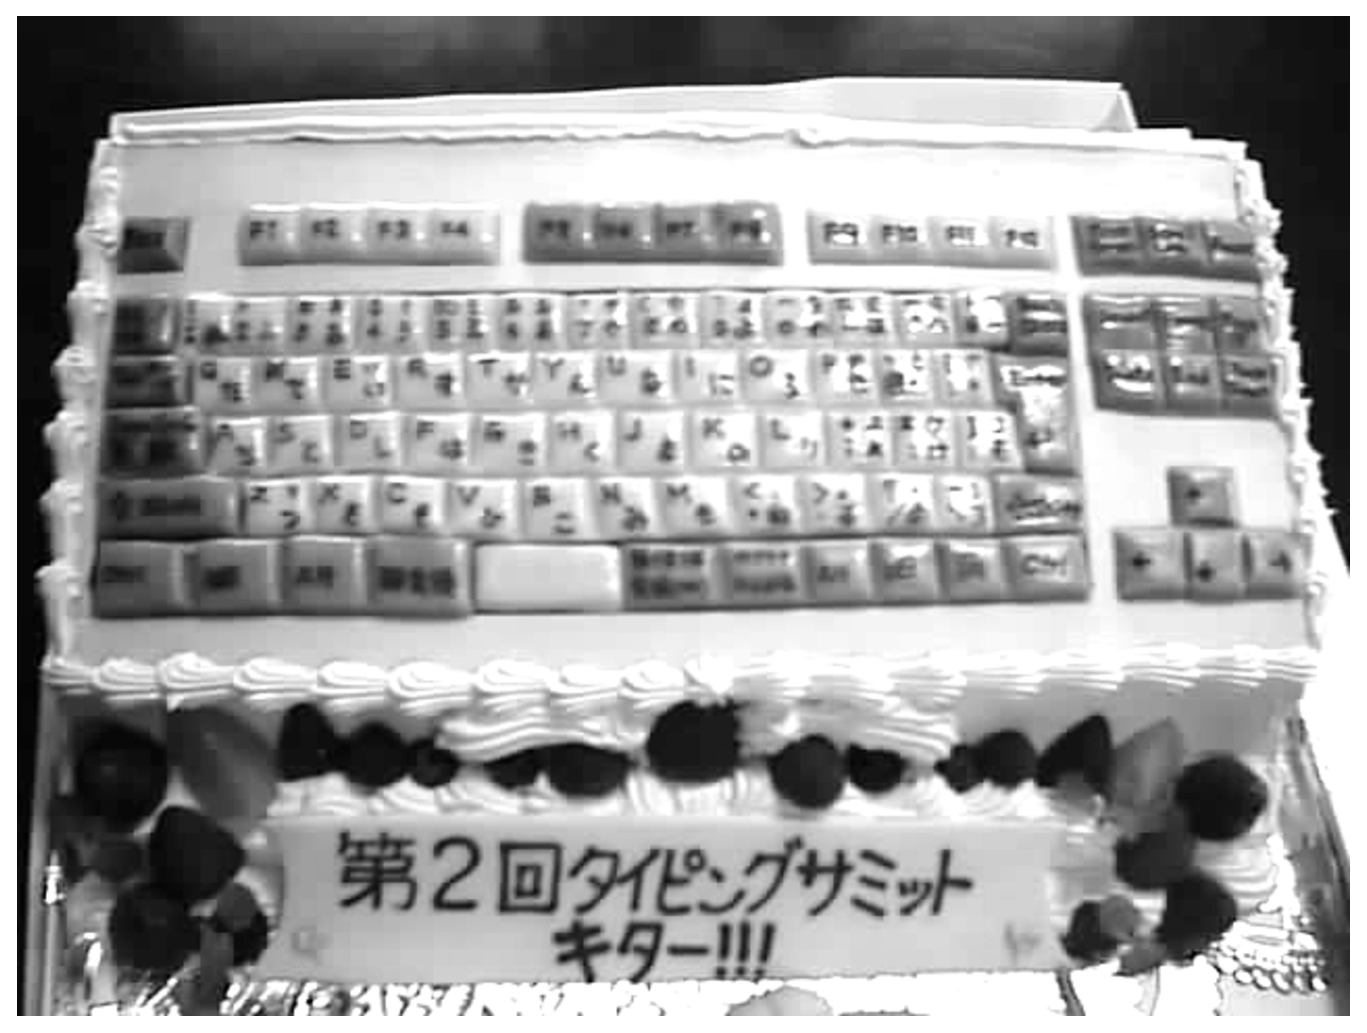
\includegraphics[width=14cm,clip]{res_x_i/typist3.eps}
 \end{center}
 \caption{タイピングサミットに持ち込まれた、キーボードケーキ。}
 \label{keycake}
\end{figure*}

\answer{むなしい}{やっぱりタイピングって普段が一人黙々とやるものだから、みんなが集まったりするのはいいよね。}

\answer{たにごん}{その時だけ TOL \footnote{月姫打ONLINE}の対戦ができるしな。あれが熱い。}

\answer{Pocari}{あーそうそう、TOL は熱い。TOL の対戦は本当おすすめですよ。}

\answer{たにごん}{あれはもっと評価されるべき。}

\answer{Pocari}{うん、もっと評価されるべき。TOD 以来最もバランスがよく整っていたゲームだった。使用キャラクターそれぞれに特性や特殊能力みたいのがあるんだけど、どのキャラにも勝てる要素がある一長一短のバランス。……そういえば当時公式の大会があって、優勝したところ、なんでも好きなものをくれるという話があって、TOLは販売停止が決まっていたので だめもとで TOL の在庫を全部下さいとお願いしてみたんです(笑)50 本くらいもらえたかな。それをウェザタイオフとかで配って、ぜひやろう、広めてねと言った。けど成果は全然。もったいない。かけあってフリーで配れたら最高なんですけど。}

\question{僕はプレイしたことありますよ。面白いですよね。}

\answer{Pocari}{タイパーオフのイベントで積極的に使うとか、そうやって広めていくしかないかなぁ。}

\question{色々思い出話を伺えたところで、話題を変えまして、最適化の話などを。}

\answer{dqmaniac}{最適化と言えば、たにごんでしょ。}

\question{たにごんさんがそもそも「最適化」という言葉をタイピングで使い始め、広めた方だと伺っています。}

\answer{Pocari}{多分それが初めだよね。}

\question{今でも最適化をした方がいいのか、使う指の本数はどうか、など議論が今なお続いているんです。}

\answer{たにごん}{指が多くて最適化するのがベストだと思う。}

\answer{Pocari}{僕もそれがいい気がするなぁ。}

\answer{たにごん}{例えば「ざ」とか同じ指じゃ絶対効率悪くて……中薬ですね。あとピアノをやっていると絶対に有利なポイントとしては、同鍵連打の時に指を変えられるということ。ピアノで「ドドドドド」ってやるときとか、指が毎回変わるから。}

\question{ピアノをやっている人だとできるんですね。}

\answer{たにごん}{うん、普通。だから「ざっきん」はこう打って(\key{Z}\key{A}を中薬で取り、\key{K}の同鍵連打を別の指で取り)、あと\key{N}は位置関係的に親指を使う。だから「ざっきん」はこんな感じで、一瞬で打てる。標準運指で「ざっきん」をこのスピードで打てることはまずない。}

\question{親指も使っているのですね。}

\answer{たにごん}{\key{N}\key{M}を親指っていうのは人から身につけた技術だなぁ。今でも素で使う。}

\answer{Pocari}{僕も親指使う時あるなぁ。あ、僕、昔は標準運指派でしたけど、今ではバリバリの最適化派です(笑)}

\question{なんと(笑)あと最適化の話題によく上がるのは、物理的なスピードで見ると最適化が有利なのはわかるのだけれども、打鍵の組立といった脳内の部分に負担がかかるのではないかという主張です。}

\answer{たにごん}{それは、もっと使えば大丈夫。}

\answer{Pocari}{うん、繰り返し練習で解消できる部分だと思う。}

\answer{たにごん}{だってもう何も考えてないから、俺。}

\question{参考にします。あと、これを聞くのは失礼にあたりそうですが、古参の皆さんならでは語れそうなこととして、年齢的な変化を伺いたいです。}

\answer{dqmaniac}{加齢による衰えというのは特に感じないですね。俺はそもそもタイピングを本格的に始めたのが 24 歳だったので。(10 年以上経った今でも)身体の限界というのは感じません。やっていないことによる退化は当然ありますが。}

\answer{Pocari}{歳を食ったからというのは半分言い訳みたいに用いられているんじゃないかなぁ。若手で(打鍵速度が)おかしい奴、僕らの代ですと Tak とかが出てくると「若い者には勝てないネー」って。身体的にみれば、タイピングってそんなに激しい運動ではないよね。例えば秒間 30 打鍵っていっても、指 8 本使って一秒に4 回打ち下ろせば32打鍵。運指を組み立てる速度の問題や、ボトルネックを(打鍵や変換の最適化で)解消する必要はあるとしても、物理的な運動限界ではないように思う。}

\answer{たにごん}{俺は今たまにタイプウェルをやると、一発で(当時の)記録を更新したりするからな。送らないけど、実力自体はまだじりじり上がってて。}

\answer{Pocari}{上がるよねぇ、やっぱり。}

\answer{たにごん}{やらないと落ちるけど。何かしらはやってるし。今でも字幕をやっている奴(字幕速記者、ステノキャプショナー)と勝負したい気持ちはあったりする。}

\answer{むなしい}{だから衰えるとしたら、単純に時間が取れないからというのが大きいかな。やっぱ社会人になって色々あると。}

\question{当時はどれくらい練習されてたんですかね。}

\answer{dqmaniac}{タイピングだけやっていた時は、平日2、3時間、休日は一日中。}

\answer{むなしい}{連休中は?}

\answer{dqmaniac}{一日中。朝から寝るまで。}

\answer{一同}{(笑)}

\answer{むなしい}{いやでも実際そうでしょ。俺もタイピングだけやってた頃は一日3、4時間は練習してた。}

\answer{Pocari}{うん、僕も暇さえあればタイピングやってた。でも練習っていう気はあんまりしていなかった。}

\answer{むなしい}{常にトライアルみたいな。やっぱりみんな2、3時間以上はやってるでしょう。そうするとやはり社会人になってからは時間的な問題はあるんじゃないかな。年齢よりは。}

\answer{Pocari}{タイプウェルは時間があればもう一回、本気でやってみたい。}

\answer{dqmaniac}{あれは時間がないとできない。社会人で忙殺されていると、時間的にもモチベーション的にも、できない。}

\answer{Pocari}{時間をかけないと伸びないから?}

\answer{dqmaniac}{伸びないね。どうしても一日一時間から一時間半くらいは現状維持をするのに必要になってしまう。でも、仕事してるとそれって無理じゃん。昔は睡眠時間削ってでも伸ばすぞーってレベルにモチベーションがあったけど、今はちょっとそこまでは無理だから。そしてタイプウェルは一週間くらいサボるとガクッと記録が落ちるから、その瞬間にやる気がなくなってしまう。でも逆に言えば、時間をかければ少しずつ確実に伸びていくので、まだ限界を感じてはいないです。いつかジジイになって時間ができた時にでも、国語 R は唯一総合 ZJ 達成してないから、そこは行きてぇなーと思ってる。}

\question{伺いたいと考えていたことは大体伺えてしまいました。あとは、若い人に伝えたいことなどがあれば。}

\answer{たにごん}{まあ、「がんばってください」しかないっすね(笑)……いやでも、根本的には何も変わってないなと思うのは、あれだけ圧倒的に速いテルと毎パソでやってもまだ勝負にはなったので、本当はもう一回タイピングに熱中したい、でも時間かかりすぎるよな……とか思っちゃう部分。あと、世界。もっと皆さん世界にチャレンジして下さい。TypeRacer はコツコツ俺もやってるけど、英文がいいと思うなぁ。Dvorak が速いとかいう説を裏付けるにもいいと思うし。世界レベルではまだまだ俺や、テルのレベルでさえ低い方だから。トップはすごいからね。やはり世界に目を向けて欲しい。}

\question{たにごんさんにそれを言って頂けると、やる気が出ます。}

\answer{たにごん}{世界に挑戦してる人って少ないからな。テルはまあ、もう国内で上に何もないから、挑戦せざるを得ないけど。}

\answer{Pocari}{実は昔から毎パソはそれをやりたがっていたんだよね。ギネス申請とかそっち方面。でも当時ギネス記録を塗り替えて載せるには、毎パソのあの形式(5 分間の実入力)の英文で 4000 文字くらい打たなくちゃいけなくて。当時さすがにそれは無理そうなスコアだったので、成立しなかった。}

\answer{たにごん}{バーバラ\footnote{タイピングのギネス記録を持つBarbara Blackburn夫人}っすか。}

\answer{Pocari}{バーバラがその基準だったのかはわからないけど。あ、バーバラと言えば、グッジョブも一度バーバラさんに連絡をつけていたよ。呼ぼうとしたんだけど、断られてしまって。}

\answer{たにごん}{歴史上の偉人だな。}

\answer{Pocari}{海外進出はやはり話題性が出てくるので、毎パソもテレビ局も興味を持っていたみたいだけど、結局どれも実現しなかった。}

\question{競技タイピング文化の隆盛・衰退というような話も、現状ですと国内のことについて言っているだけですからね。}

\answer{たにごん}{世界の壁は厚いよ。TypeRacer で遊んでても、基本的にはずっと勝てるけど、時々速い奴が紛れ込んでくるとボコられる。一時間打って 180 wpm\footnote{英語圏での WPM は、5 倍すると日本語圏(e-typing)の WPM。}くらいが最高で出るところに、毎回 185 wpm とかガンガン出してくる奴とかがいて。勝てないっていう。毎回だからなぁ……俺もテルも F5 でキャンセルしないクチだから、平均スコアが伸びにくいんだよ。でもそいつも全然キャンセルしないのに、平均スコアがおかしなゾーンに入ってる。160 wpm 超とか。}

\answer{Pocari}{それは Sean Wrona\footnote{TypeRacerのトップランカー。米国のタイピング大会で優勝するなどの実績を持ち、現役のタイピング競技者では世界一ではないかと噂されている方。}とは違う人?}

\answer{たにごん}{いや Sean だけど、彼だけじゃないよ。ヤバい奴がいっぱい。Julian とかもみんな頭おかしい。}

\answer{Pocari}{たにごんは何位くらいなの?}

\answer{たにごん}{3 ページ目くらいだから……二十何位かな。}

\answer{Pocari}{マジで!?}

\answer{たにごん}{俺もテルも 1 ページ目に入るにはほど遠い。まず俺らのベストスコアが全く及んでないから。そのベストスコア付近にアベレージを置いている連中というのは頭がおかしい。出たことのないスコアをアベレージに置かれるというあの絶望感はすごい。}

\answer{Pocari}{タイプウェルでいうと、Possibleがアベレージですみたいな状況ね……。}

\answer{たにごん}{でもあれは目標にするにはいい。ちゃんと実用だし。シフトキーも押さないといけないし。}

\question{TypeRacer 推しということですね。}

\answer{たにごん}{TypeRacer 推し。他のもあったらそれが一番いいんだけど、今のところ TypeRacer が一番キャッチーな感じ。適度な長さといい。}

\question{Pocari さんからは何かありますか。}

\answer{Pocari}{僕も世界指向はいいと思う。その他だと、今のコミュニティをもっと広め、盛り上げてほしい、というのがあるかな。}

\answer{たにごん}{タイピング界というものが存在するのかどうかが怪しくなってきているよね、今は。}

\answer{Pocari}{まあね。一人一人はもちろん今も昔も変わらず情熱的にタイピングをやっていると思うんだけど、昔のむなしいみたいな存在というか、コミュニティを広める方向に活動している人はあんまりいない気がする。}

\question{むなしいさん並にオフ会を企画したり、団体を実際に作ってしまうようなレベルの貢献をする人というのは、あまりいないですね。}

\answer{Pocari}{うん。TODとかグッジョブみたいな話は外から来た話だから、どうしようもないけれど、形成されたコミュニティがそれを呼ぶ、というのもあるんじゃないかな。実際、全タ連宛に問い合わせがくることは今もある。僕らがオフ会をやらなくなってしまったのは、なんでかというと……。}

\answer{dqmaniac}{ゲーセンから TOD がなくなっていったから、というのはひとつある。}

\answer{むなしい}{一番は新鮮味がないからじゃない。もう特に会いたい人とかがいるわけではないし。}

\answer{Pocari}{当時は見てみたかったんだよね、他の人がどうやって打っているのか。}

\answer{dqmaniac}{あとはガチで対戦したかった。今はもうやっても大体結果がわかってしまっているんだよな。例えば、ぽかたんが俺とローマ字で対戦しても 100\% ぽかたんが勝つでしょう。}

\answer{Pocari}{逆に、今最前線のタイパーがそういった活動にあまり積極的じゃないところを不思議に思うこともある。}

\question{ネットで対戦ができてしまうですとか、YouTube のような動画サイトですごい人の手元なども見ることができてしまう、というのはひとつあると思います。dqmaniac さんはどうでしょう。}

\answer{dqmaniac}{似たようなものだけど、「TOD 対戦やろうぜ」と伝えたい。俺は決して興味を失ったわけじゃないので。9 月に 10 周年オフをやった時にもちょっと燃えるものがあって、最近毎日 DC 版 TOD 打ってますよ。ドリルモードも今やって更新したりしてるんで、対戦を望む人がいるならいつでも受けて立ちます。ローマ字じゃトップレベルの人とやったら話にならんかもしれないが、かな入力だったらある程度は戦えるはずだから。}

\question{大分まとまってきました。最後に文化的な話として、タイピング界の過去から現在・未来を考えるとき、世代間での情報断絶があると思うんです。今回お話頂いたようなことも、よくよく頑張って調べれば web 上から探して来ることができるのかもしれませんが、これだけまとまった形で把握することは至難だと思います。実際、若い我々が考えているようなことも、かつての常識の再発見であったりすることがあるわけです。こうした状況を改善し、効率化していけたらと思うのですが。}

\answer{Pocari}{これは、今も昔も同じ状況なんじゃないかな。例えば Twitter でつぶやかれた情報は、フォロワー且つタイムラインを見ていた人には届くし、RTやTogetterで多少は拡散されると思うけれど、世代間で伝達されうる情報かというと、そうじゃない。三年後にそのツイートを追えと言われても無理な話でしょ。今現役の人には伝わるから、情報共有できている感じがあるけれど、そのままじゃ後世には残らない。}

\question{今僕らが上の世代との間に感じているような情報の壁は、このままではやはり次の世代に対しても存在してしまう、ということですね。}

\answer{Pocari}{そう。僕らの世代では(現世代から見れば情報が残りにくいように思う)掲示板やオフで情報交換をしてたわけだけど、当時の僕らの感覚としては「必要な情報は周知・共有できている」と思ってた。同じ感覚じゃないかな。情報をまとめるって、本人たちにとっては現役にいる間は必要性が薄いから、なかなかやらない。}

\answer{dqmaniac}{TODの攻略情報に関しては俺のホームページ\footnote{\url{http://www.geocities.jp/dqmaniac/}}に結構まとめてあるよ。}

\answer{Pocari}{dq さんは文章をまとめるスキルとしても、ポジション的にもまとめられる人だから、いろいろと記録を残してくれているよね。難しいのは、まとめる能力がある人と、発言の影響力がある人というのが必ずしも同じじゃないという点。影響力のある人が、まとめる能力も高いと、必然的に情報はちゃんと蓄積されていく。でも仮に、当時僕や dq さんの発言や日記に書かれていた内容を、(タイプウェルのレベルにして)SS くらいのタイパーがまとめようとした場合、それってかなりやりづらいんじゃないかな。どの世界でも同じだと思うけれど、まとめる人にも一定のスキルを求めてしまう。そうじゃないと納得感がないというか……。}

\answer{dqmaniac}{そうですね。そういう意味では俺もやりづらいかな。例えば今のタイプウェルのトップレベルの人達がやっているような練習法を、俺が持ってきて日記にまとめる……なんてこともちょっと(心理的に)やりづらい。}

\answer{Pocari}{その時その時で発言力のある人、影響力のある人というのは必然的にトップタイパーになると思うので、そういう人が主導してくれないと難しいと思う。その点、今回の本みたいな合作は良いよね。例えば、僕が現役だった頃にタイプウェル攻略法を書けと言われても、たにごんを意識してしまって僕一人では心理的に厳しかったと思う。でも、たにごんと一緒に二人でならそういう障害はなくなる。}

\answer{dqmaniac}{今は「タイパー辞典」とかあるじゃない。あそこを Wikipedia チックに改修していってまとめるというのはどうだろう。}

\question{本当に不特定多数が書ける場所だと、誰でも書けるがゆえに、誰も書かない……という状況がよくあると思っています。あとはいわゆる民度の問題も。Wikipedia の場合は参加者のレベルが相当に高いので、中に一部おかしな人が紛れていても、他の大勢が理知的で客観的に判断を下していくので問題はそう起きないと思うんですけど。}

\answer{dqmaniac}{せっかく書いても、心ない人達がガーッて消しちゃったりとかするわけだよね。}

\question{しかし一方誰かが責任を持ってやろうとすると、やはり叩かれて難しいですよね。先ほど出た「複数人で」というのを取り込んで、不特定多数ではない複数人で共同編集していくというのは現実解かなと思ってはいるんですが。}

\answer{Pocari}{全員が納得する文章は絶対に書けない。ちょっと偏った意見になっても、間違った部分があっても、それを割り切った上で数名で書いていった方が、体系的な内容になる気がするな。責任がある程度どこかにあった方が綺麗にまとまるんだと思う。}

\answer{dqmaniac}{まあそうした試みの一つの形が今回のこの本であり、このインタビュー企画なわけでしょう。}

\question{そう評価して頂けると光栄です。気持ちとして、一つ下の世代に向けて整備らしきことができたら良いなとは思っています。今この時期を逃すと Pocari さんら第一世代から情報を聞き出すということも次第に難しくなると思ったので、今回お話が聞けて本当に良かったです。}

\answer{Pocari}{いえいえ、僕たちも、こういう機会であったり、オフ会であったり、誘ってもらえればまだまだ積極的に参加しますよ。古参と呼ばれる人々も。たぶん想像されているほどタイピングと離れてはいない。もっとつながりがあってもいいなとも、思っていますし。}

\answer{dqmaniac}{さっきも言ったけど「TOD 対戦やろうぜ」と(笑)}

\question{皆さん、大変有意義なお話をありがとうございました。}
